% =============================================================================
% Subset-Decomposed Evaluation of Schema-Aware Grounding in NL2GeoSQL
% Computers & Geosciences submission -- manuscript with author details
% =============================================================================
\documentclass[11pt]{article}

\usepackage[margin=1in]{geometry}
\usepackage{times}
\usepackage{amsmath,amssymb}
\usepackage{graphicx}
\usepackage{booktabs}
\usepackage{multirow}
\usepackage{caption}
\usepackage{subcaption}
\usepackage{enumitem}
\usepackage{url}
\usepackage[authoryear,round]{natbib}
\usepackage[hidelinks]{hyperref}
\usepackage{tikz}
\usetikzlibrary{positioning,arrows.meta,shapes.geometric,fit,calc}
\usepackage{algorithm}
\usepackage{algorithmic}
\setlength{\emergencystretch}{2em}

\title{Schema-Aware Grounding Effects in PostGIS\\
       Natural-Language-to-SQL: A Subset-Decomposed Evaluation Across Eleven LLMs}
\author{Ning Zhou\\
\textit{Beijing SuperMap Software Co., Ltd., Beijing, China}\\
ORCID: \href{https://orcid.org/0009-0002-5647-7388}{0009-0002-5647-7388}\\
Corresponding author: \href{mailto:zhouning1@supermap.com}{zhouning1@supermap.com}}
\date{}

\begin{document}
\maketitle

% =============================================================================
\begin{abstract}
% =============================================================================
Natural-language interfaces to spatial databases increasingly use schema-aware
grounding: prompt-side evidence about table aliases, geometry columns, spatial
reference systems, PostGIS operators, value hints, and safety constraints. For
computational geoscience applications, this is a spatial-database informatics
problem rather than only a language-model benchmarking problem. We evaluate
grounding as an intervention on CQ-125, a 125-question Chongqing PostGIS
benchmark containing 85 spatial-query questions and 40 robustness questions,
across 11 LLM families with $N{=}3$ paired samples per family. All paired tests
use question-level majority vote across the stochastic samples followed by a
single exact two-sided McNemar test, avoiding the pseudoreplication that results
from treating $NQ$ repeated samples as independent observations. Grounding
produces a subset-dependent pattern. On the Robustness subset, all 11
families improve in point estimate ($+12.50$ to $+65.00$ pp; nine significant in
unadjusted per-cell tests and after Holm correction within the Robustness
comparison set, one marginal, one non-significant positive). On the Spatial
subset, 7 families show unadjusted significant positive gains ($+11.76$ to
$+23.53$ pp), 2 show marginal positive gains, and 2 show non-significant negative
point estimates; Holm correction within the Spatial comparison set leaves 3
positive cells significant. The most negative panel estimate is \texttt{gemini-3.5-flash}
($\Delta=-10.59$ pp, $p=0.136$), and a balanced $N{=}5$ focused check on the
same family retains this negative but non-significant Spatial point estimate.
We therefore make a bounded claim: subset
decomposition and de-pooled paired testing are necessary for defensible
grounding-effect evaluation in geospatial NL2SQL; cross-family effects are
heterogeneous; and the observed negative tail requires out-of-benchmark
replication before it can be treated as a stable model-family property.
\end{abstract}

\noindent\textbf{Keywords:} NL2GeoSQL; PostGIS; semantic grounding; spatial-SQL execution accuracy; LLM evaluation; subset analysis; paired statistical testing; large language model.

% =============================================================================
\section{Introduction}
\label{sec:intro}
% =============================================================================

Natural language access to spatial databases is a long-standing GIScience problem~\citep{goodchild1992gis,egenhofer1991topological,clementini1993small}. Recent large language models have advanced general text-to-SQL on benchmarks such as Spider~\citep{yu2018spider} and BIRD~\citep{li2023bird}; PostGIS-based NL2GeoSQL adds the OGC Simple Feature Access predicates~\citep{ogcsfs}, coordinate-reference-system transformations, the \texttt{geometry}/\texttt{geography} type distinction, KNN operators, and the safety constraints any production GIS must enforce~\citep{postgis}. These requirements make geospatial text-to-SQL a GIScience problem as well as a language-model problem: the system must translate geographic concepts into executable spatial predicates while preserving units, coordinate reference assumptions, result shape, and read-only behaviour.

The standard engineering response is \emph{schema-aware grounding}: an upstream stage that injects table aliases, value enumerations, geometry-type metadata, SRID flags, large-table boundedness rules, and PostGIS dialect cues into the LLM prompt. Grounding is often evaluated as a single positive intervention, but this aggregate view is too coarse for mixed geospatial benchmarks. A benchmark that combines ordinary spatial queries with robustness cases is not testing one homogeneous capability. Spatial questions reward precise predicate choice, join structure, geometry measurement, and output-shape control; robustness questions reward refusal, schema enforcement, and bounded execution. The same grounding context can therefore interact differently with each subset.

This paper evaluates that interaction on CQ-125, a 125-question Chongqing PostGIS benchmark containing 85 spatial-query questions and 40 robustness questions. Across 11 LLM families at $N{=}3$ paired samples per family, grounding has uniformly positive point estimates on Robustness ($+12.50$ to $+65.00$ pp). On Spatial, however, effects are heterogeneous: seven families improve in unadjusted per-cell tests, two are marginal positive, and two have non-significant negative point estimates; after Holm correction within the 11 Spatial tests, three positive cells remain significant. The most negative panel estimate is \texttt{gemini-3.5-flash} ($-10.59$ pp, $p=0.136$). A balanced $N{=}5$ three-condition analysis on the same family, using no-grounding, grounding-only, and grounding plus a minimal prompt patch, retains the same Spatial grounding-only point estimate ($-10.59$ pp, $b/c=19/10$, $p=0.136$) and a large Robustness gain ($+27.50$ pp, $p=0.001$). The stable conclusion is therefore not that grounding generally hurts. It is that grounding effects are subset-conditional and family-conditional, and that aggregate execution accuracy can hide the interaction.

\medskip
\noindent\textbf{Contributions.}
\begin{enumerate}[leftmargin=*]
  \item \textbf{Methodological (\S\ref{sec:gisr:methodology}).} Aggregate execution accuracy is insufficient for grounding-effect claims on geospatial NL2SQL when robustness and spatial questions are mixed. The paired-test convention also matters: pooling $N$ stochastic samples $\times$ $Q$ questions into a single McNemar test on $NQ$ observations violates independence and inflates significance. We use question-level majority vote across $N$ samples followed by a single exact two-sided McNemar test on the per-question table.
  \item \textbf{Empirical (\S\ref{sec:gisr}).} On 11 LLM families surveyed at $N{=}3$ on CQ-125, grounding improves Robustness in all families by point estimate, but Spatial effects range from $-10.59$ to $+23.53$ pp. This establishes cross-family heterogeneity rather than a universal positive or negative effect.
  \item \textbf{Diagnostic and design implication (\S\ref{sec:gisr:minimod}--\S\ref{sec:gisr:routing}).} For \texttt{gemini-3.5-flash}, a focused three-condition analysis identifies a candidate negative-tail case and links many regressions to unsolicited SQL elaboration. A perfect-classifier routing calculation gives an upper bound for subset-conditional grounding, but we treat it as a design implication, not a validated production policy.
\end{enumerate}

The semantic-layer framework, intent-conditioned router, SQL postprocessor, and execution-time self-correction loop on which grounding is implemented are described in \S\ref{sec:method}. The new questions are not how to ground, but \emph{when grounding helps which question class on which family} and \emph{how to test that question with an honest paired statistic}. As supporting deployment context, not as primary inferential evidence, \S\ref{sec:gemma4-scale-sweep} reports a fixed-host Gemma4 model-size sweep.

The paper proceeds as follows. \S\ref{sec:related} reviews GIScience foundations and recent NL-to-spatial-database systems. \S\ref{sec:method} summarises the framework. \S\ref{sec:experiments} describes the experimental setup. \S\ref{sec:baseline-results} reports framework behaviour and bridges to \S\ref{sec:gisr}, the central empirical section. \S\ref{sec:discussion} discusses interpretation, limitations, and ties to GIScience. \S\ref{sec:conclusion} concludes.

% =============================================================================
\section{Related Work}
\label{sec:related}
% =============================================================================

% Content of §2 Related Work: section header is in the master file.

\subsection{GIScience foundations for NL-to-spatial-database}

Natural language access to spatial databases sits within the GIScience programme articulated by \citet{goodchild1992gis}: formalising geographic concepts so they can be computed rigorously. The relational semantics we ground against trace to the $4$- and $9$-intersection formalisms~\citep{egenhofer1991topological}, the end-user topological relations of \citet{clementini1993small}, OGC Simple Feature Access~\citep{ogcsfs}, and GeoSPARQL~\citep{ogcgeosparql}. PostGIS~\citep{postgis} operationalises these ideas in PostgreSQL through geometry/geography types, casts, metric and topological functions, coordinate transformations, and KNN operators. Our grounding rules expose these constraints as prompt-side evidence.

\subsection{Natural language interfaces to spatial databases}

Early geospatial question answering focused on small fact databases: \citet{zelle1996geoquery} used inductive logic programming for GeoQuery, and \citet{punjani2018geospatial} extended this to template-based question answering over linked geospatial data, highlighting spatial-predicate coverage and coordinate-system awareness. Recent LLM-era work falls into two groups. The first targets end-to-end NL-to-executable-spatial-SQL: NALSpatial~\citep{liu2025nalspatial} translates user queries into spatial SQL (implemented over the SECONDO spatial DBMS rather than PostGIS); Monkuu~\citep{yu2025monkuu} is an IJGIS-published LLM-powered NL interface with dynamic schema mapping; GeoSQL-Eval~\citep{hou2026geosql} contributes a large-scale LLM evaluation on PostGIS functions and NL2GeoSQL tasks. The second targets higher-level GeoAI agents: GeoCogent~\citep{houcoding2025} is an LLM-based agent for geospatial code generation; GeoAgent~\citep{lin2026geoagent} is a hierarchical multi-agent architecture. Surveys map the broader opportunities~\citep{mai2024foundation}.

Our contribution is narrower than a general GeoAI agent and different from a function-coverage benchmark. We study grounding as an intervention in end-to-end execution-graded NL-to-PostGIS-SQL, where the semantic layer encodes OGC predicates, SRIDs, geography casts, KNN operators, and read-only bounded-output constraints. Compared with NALSpatial and Monkuu, we add a 125-question execution benchmark with an explicit Robustness suite, question-level McNemar testing, and an 11-family grounding-effect panel. Compared with GeoSQL-Eval, CQ-125 is smaller but designed for paired intervention analysis rather than broad function inventory.

Table~\ref{tab:related-comp} summarises the distinction.

\begin{table}[t]\centering\footnotesize
\caption{Direct comparison with recent NL-to-spatial-database systems. NALSpatial is implemented over SECONDO, not PostGIS. $\checkmark$: supported / reported; $-$: not reported.}
\label{tab:related-comp}
\setlength{\tabcolsep}{3pt}
\begin{tabular*}{\textwidth}{@{\extracolsep{\fill}}lccccc@{}}
\toprule
System & E2E & Function & Safety & Paired gnd. & Released \\
\midrule
Our framework                          & $\checkmark$ & $-$           & $\checkmark$ & $\checkmark$ & $\checkmark$ \\
NALSpatial~\citep{liu2025nalspatial}    & $-$           & $-$           & $-$           & $-$           & $\checkmark$ \\
Monkuu~\citep{yu2025monkuu}             & $\checkmark$ & $-$           & $-$           & $-$           & $-$           \\
GeoSQL-Eval~\citep{hou2026geosql}       & $-$           & $\checkmark$ & $-$           & $-$           & $\checkmark$ \\
GeoCogent~\citep{houcoding2025}         & $-$           & $-$           & $-$           & $-$           & $-$           \\
GeoAgent~\citep{lin2026geoagent}        & $-$           & $-$           & $-$           & $-$           & $-$           \\
\bottomrule
\end{tabular*}
\end{table}

\subsection{Text-to-SQL with LLMs and semantic layers}

LLM text-to-SQL has progressed through Spider~\citep{yu2018spider,rajkumar2022evaluating}, BIRD~\citep{li2023bird}, Spider~2.0~\citep{lei2025spider2}, and BEAVER~\citep{chen2024beaver}. DIN-SQL~\citep{pourreza2023dinsql} decomposes prompting into schema linking, classification, generation, and self-correction; DAIL-SQL~\citep{gao2024dail} uses skeleton-similarity few-shot selection; C3~\citep{dong2023c3} studies calibrated zero-shot prompting; CSpider~\citep{min2019cspider} is an early multilingual benchmark. Semantic-layer tools such as MetricFlow~\citep{metricflow} encode entities, measures, dimensions, and metric graphs for analytical warehouses. We adapt that vocabulary with GIS annotations, and use BIRD as a supporting warehouse track of the bilingual framework.

% =============================================================================


% =============================================================================
\section{Method: Semantic-Layer Framework}
\label{sec:method}
% =============================================================================

% Content of §3 Method: section header is in the master file.

\subsection{Formal scope: semantic layer as metadata graph \texorpdfstring{$G=(V,E)$}{G=(V,E)}}
\label{sec:formal-scope}

We formalise the semantic layer as a directed multigraph $G = (V, E)$ that encodes the executable subset of OGC Simple Feature Access~\citep{ogcsfs} required for PostGIS grounding. $V = E_{geo} \cup D \cup M \cup I \cup P \cup C$ where $E_{geo}$ are geographic-entity (PostGIS table) vertices with attributes (geometry column, SRID, geometry type); $D, M$ are dimension/measure vertices for the warehouse track; $I$ are intent tags (\texttt{attribute\_filter}, \texttt{aggregation}, \texttt{spatial\_join}, \texttt{spatial\_measurement}, \texttt{knn}, \texttt{preview\_listing}); $P$ are OGC SFA predicate vertices partitioned into topological, metric, and KNN classes; $C$ are constraint vertices for SRID ranges, unit rules, and safety/refusal. $E$ comprises $E_{hasGeom}, E_{fk}, E_{topo}, E_{metric}, E_{knn}, E_{route}, E_{safety}, E_{unit}$ (table--geometry, foreign keys, predicate--entity edges, intent$\to$predicate routing, refusal edges, and SRID range$\to$required cast$\to$yielded unit chains). Algorithm~\ref{alg:build-graph} materialises $G$ at agent startup from the live PostGIS catalog. $G$ is an \emph{executable subset} of the OGC SFA predicate taxonomy, not a complete geospatial ontology; full GeoSPARQL/ISO~19107 alignment is future work, and Table~\ref{tab:alignment} documents the rule-level mapping we currently enforce.

\begin{algorithm}[t]
\caption{\textsc{BuildSemanticGraph}($\mathit{schema}, \mathit{prefix}$)}
\label{alg:build-graph}
\begin{algorithmic}[1]
\STATE $G \gets$ empty multigraph
\FOR{$(t, c, \mathit{srid}, \tau) \in$ \texttt{geometry\_columns}}
  \IF{$t$ starts with $\mathit{prefix}$ and $\mathit{srid} \neq 0$}
    \STATE add GEO\_ENTITY vertex $(t, c, \mathit{srid}, \tau)$
  \ENDIF
\ENDFOR
\FOR{$(t_s, t_t) \in$ \texttt{key\_column\_usage}}
  \STATE add edge $(t_s \to t_t, \text{FK})$
\ENDFOR
\STATE register topological / metric / KNN predicate vertices (OGC SFA 06-104r4)
\STATE register intent vertices; route intents $\to$ predicate classes
\STATE register unit-rule edges: metric $\to$ SRID range $\to$ required cast
\RETURN $G$
\end{algorithmic}
\end{algorithm}

\begin{table}[t]
\centering\footnotesize
\caption{Alignment of semantic-layer rules to OGC SFA~\citep{ogcsfs}, ISO 19107~\citep{iso19107} clauses, and PostGIS functions~\citep{postgis}. Rule-level mapping; each enforced rule traces to a specific clause.}
\label{tab:alignment}
{\setlength{\tabcolsep}{4pt}
\begin{tabular}{@{}lllll@{}}
\toprule
Rule & Edge class & OGC 06-104r4 clause & ISO 19107 clause & PostGIS \\
\midrule
\texttt{R\_topo\_intersects} & $E_{topo}$ & \S 6.1.2.3 (Relate)   & \S 6.2.2 & \texttt{ST\_Intersects} \\
\texttt{R\_topo\_contains}   & $E_{topo}$ & \S 6.1.2.3 (Relate)   & \S 6.2.2 & \texttt{ST\_Contains} \\
\texttt{R\_topo\_within}     & $E_{topo}$ & \S 6.1.2.3 (Relate)   & \S 6.2.2 & \texttt{ST\_Within} \\
\texttt{R\_metric\_length\_geog}   & $E_{unit}$ & \S 6.1.2.3 (Length) + \S 8.2.3 & \S 6.4.14 & \texttt{ST\_Length(geog)} \\
\texttt{R\_metric\_area\_geog}     & $E_{unit}$ & \S 6.1.2.3 (Area) + \S 8.2.3   & \S 6.4.15 & \texttt{ST\_Area(geog)} \\
\texttt{R\_metric\_dwithin\_geog}  & $E_{unit}$ & \S 6.1.2.3 (Distance) + \S 8.2.3 & \S 6.4.10 & \texttt{ST\_DWithin(geog)} \\
\texttt{R\_knn\_nearest}     & $E_{knn}$  & \S 6.1.2.3 (Distance) & \S 6.4.10 & \texttt{<->} KNN \\
\texttt{R\_safety\_refusal}  & $E_{safety}$ & not in OGC & --- & postprocessor AST \\
\texttt{R\_safety\_bounded}  & $E_{safety}$ & not in OGC & --- & \texttt{LIMIT} injection \\
\bottomrule
\end{tabular}
}
\end{table}

\subsection{Problem formulation}

We formulate cross-domain natural language to SQL as the task of translating a user question $q$ into an executable SQL statement $s$ over heterogeneous structured databases that may belong to either geospatial or conventional warehouse domains. Let $S$ denote the executable schema representation extracted from the database catalog, and let $E$ denote semantic-side evidence such as aliases, hierarchy expansions, geometry metadata, value hints, or fact/dimension/entity annotations. The problem can then be written abstractly as
\begin{equation}
  \hat{s} = f(q, S, E),
\end{equation}
where $f$ is implemented by an LLM-conditioned generation pipeline rather than a single end-to-end model. Unlike standard text-to-SQL settings, the target databases in our problem formulation are not assumed to share homogeneous operator semantics. In warehouse-style databases, correct SQL generation primarily depends on schema linking, join reasoning, aggregation, and temporal filtering. In geospatial databases, however, the model must additionally reason about geometry-bearing columns, spatial relations, coordinate systems, and domain-specific operators such as intersection, containment, buffering, and area or distance calculation. The purpose of our framework is therefore not only to generate valid SQL, but also to provide a semantic mediation layer that adapts the grounding process to the structural characteristics of each domain.

\subsection{Three-stage pipeline}

We design NL2Semantic2SQL as a three-stage pipeline (Figure~\ref{fig:arch}). In the first stage, the system performs semantic resolution over a semantic layer that stores table-level and column-level annotations, aliases, domain hints, and task-relevant metadata. In the second stage, the resolved information is combined with database schema inspection and optional few-shot retrieval to construct a grounded context block for SQL generation. In the third stage, the generated SQL is postprocessed, executed under safety constraints, and, when necessary, revised through an execution-feedback self-correction loop. This decomposition separates semantic interpretation from SQL synthesis, allowing the framework to expose domain-specific evidence to the language model while keeping the final generation step constrained by executable schema information.

\begin{figure}[t]
\centering
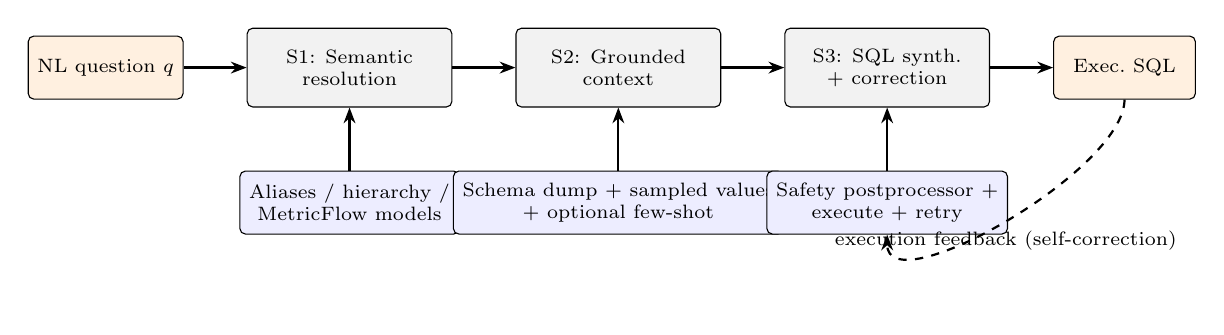
\begin{tikzpicture}[
  node distance=8mm and 8mm,
  every node/.style={font=\small},
  stage/.style={draw, rounded corners=2pt, minimum width=26mm, minimum height=10mm, align=center, fill=gray!10, font=\scriptsize},
  block/.style={draw, rounded corners=2pt, minimum width=26mm, minimum height=8mm, align=center, fill=blue!7, font=\scriptsize},
  io/.style={draw, rounded corners=2pt, minimum width=18mm, minimum height=8mm, align=center, fill=orange!12, font=\scriptsize},
  arrow/.style={-{Stealth[length=2mm]}, thick}
]
\node[io]    (q)    {NL question $q$};
\node[stage] (s1) [right=of q]   {S1: Semantic \\ resolution};
\node[stage] (s2) [right=of s1]  {S2: Grounded \\ context};
\node[stage] (s3) [right=of s2]  {S3: SQL synth.\ \\ + correction};
\node[io]    (sql) [right=of s3] {Exec.\ SQL};

\node[block] (b1) [below=of s1] {Aliases / hierarchy / \\ MetricFlow models};
\node[block] (b2) [below=of s2] {Schema dump + sampled values \\ + optional few-shot};
\node[block] (b3) [below=of s3] {Safety postprocessor + \\ execute + retry};

\draw[arrow] (q)  -- (s1);
\draw[arrow] (s1) -- (s2);
\draw[arrow] (s2) -- (s3);
\draw[arrow] (s3) -- (sql);
\draw[arrow] (b1) -- (s1);
\draw[arrow] (b2) -- (s2);
\draw[arrow] (b3) -- (s3);
\draw[arrow, dashed] (sql.south) .. controls +(0,-9mm) and +(0,-9mm) .. node[below, font=\scriptsize]{execution feedback (self-correction)} (b3.south);
\end{tikzpicture}
\caption{Architecture of NL2Semantic2SQL: Stage~1 semantic resolution, Stage~2 grounded-context assembly, Stage~3 SQL synthesis with postprocessor and self-correction.}
\label{fig:arch}
\end{figure}

\subsection{Geospatial-aware grounding and bilingual routing}

The framework's geospatial path explicitly identifies geometry columns, geometry types, and spatial reference information, and injects operator-level rules into the grounding context. These rules distinguish topological from metric predicates and specify when area or distance calculations require coordinate transformation or geography casting, reducing the burden on the language model to infer execution constraints from raw schema text. When spatial signals are absent, the framework falls back to generic schema linking and aggregation-oriented prompt construction. Routing between these paths is driven by a bilingual intent classifier that recognises Chinese GIS keywords (spatial operator terms, Chinese administrative region names, Chinese measurement units) alongside English warehouse expressions (``how many'', ``average'', ``compare''). In real-world deployments GIS analysts often query in Chinese while warehouse analysts use English, and a single interface must handle both without language-specific model swapping; bilingual routing is therefore a first-class design choice rather than an afterthought.

\subsection{Warehouse-side enhancements}

For non-geospatial warehouse queries, the framework adds three domain-adaptive enhancements. \emph{Cross-domain candidate ranking} reprioritises sources based on whether the parsed semantic context contains spatial operators or region filters; when such signals are absent, geometry-bearing tables are deprioritised and tables with matched column evidence are boosted. \emph{Value-aware grounding} injects sample distinct values from low-cardinality text columns so that the model can use exact categorical values rather than hallucinated strings. \emph{MetricFlow-style fact/dimension modelling} stores per-table roles, entity columns (primary or foreign join keys), and measure columns in a semantic-model registry; at grounding time, candidate tables are matched against this registry and explicit join-path hints are derived by aligning shared entities across fact/dimension pairs. These hints are injected only for non-spatial queries, leaving the GIS path unchanged.

\subsection{Execution-time self-correction}

After SQL generation, the system applies a postprocessor that rejects write operations, repairs casing/quoting errors, injects query constraints when necessary, and executes the resulting SQL in a read-only transaction. If execution fails, the framework enters a bounded self-correction loop. Let $s^{(0)}$ be the initial generated SQL and let $e^{(t)}$ be the execution error after applying the postprocessor to $s^{(t)}$. The retry policy is:
\begin{equation}
  s^{(t+1)} = g\big(q, s^{(t)}, e^{(t)}, S\big), \quad t = 0,1,\dots,T-1,
\end{equation}
where $g$ is a fast corrective LLM call and $T$ is the maximum retry count (in our implementation, $T=2$). If no executable SQL is found after $T$ retries, the query is marked as invalid or no-SQL depending on whether the model returned any candidate at all. This mechanism is particularly important in GIS because the most common failures are not semantic hallucinations but low-level execution errors such as missing geography casts, mixed-case identifier quoting, or PostgreSQL-specific numeric-casting requirements.

\subsection{Worked example: end-to-end PostGIS grounding}
\label{sec:worked-example}

A worked example tracing a Chongqing benchmark question (length-of-one-way-roads in km) through every pipeline stage --- including the \texttt{::geography} cast injected by Stage~2, the unit-conversion rule, the postprocessor's row-shape sanity check, and the resulting execution-based match against the gold SQL --- is provided in Supplement~S2. Three implementation artefacts support the flow: a per-database YAML semantic layer (table aliases, geometry columns with SRID, rule identifiers); a small intent-rule set (\texttt{attribute\_filter}, \texttt{aggregation}, \texttt{spatial\_join}, \texttt{spatial\_measurement}, \texttt{knn}, \texttt{preview\_listing}, each associated with a minimal set of prompt-side rules); and the postprocessor (write-node rejection, identifier repair against the real schema, large-table \texttt{LIMIT} injection, the execution-time retry loop above). The anonymised companion repository releases minimal versions of all three.

\subsection{Multi-track evaluation protocol}

Evaluation is performed on three benchmark tracks. The geospatial track uses the 125-question GIS benchmark (85 Spatial + 40 Robustness), covering spatial selection, overlap analysis, metric distance queries, buffering, spatial aggregation, and a dedicated robustness suite that probes refusal behaviour on dangerous, illusory, schema-mismatched, and out-of-memory requests. The warehouse track uses BIRD mini\_dev~\citep{li2023bird} with two disjoint subsets: a 108-question design set and a 150-question independent held-out set, both evaluated in single-pass mode. The cross-lingual track pairs 50 Chinese-translated BIRD questions with 50 native-Chinese GIS questions. For all tracks we use execution accuracy (EX) as the primary metric: a prediction is correct if and only if its execution result set matches the gold SQL under set-equality with numeric tolerance. We additionally report 95\% Wilson confidence intervals, execution validity, per-difficulty breakdowns, paired McNemar tests (two-sided exact binomial), and token cost. Concrete sample sizes and the construction of each track are described in Section~\ref{sec:experiments}.

% =============================================================================


% =============================================================================
\section{Experimental Setup}
\label{sec:experiments}
% =============================================================================

% Content of §4 Experimental Setup: section header is in the master file.

\subsection{Experimental setup}

\noindent\textbf{Evaluation protocols.} The primary analysis is the CQ-125 grounding-effect study in \S\ref{sec:gisr}: no-grounding (A) versus grounding-only (B) across 11 LLM families, with $N{=}3$ paired samples and question-level majority-vote McNemar tests. A focused \texttt{gemini-3.5-flash} diagnostic adds grounding plus minimal-modification rules (C) and uses a balanced A/B/C design with $N{=}5$. Table~\ref{tab:protocol-inventory} separates this inferential panel from supporting framework, deployment, and harness-readiness results.

\begin{table}[t]
\centering
\footnotesize
\caption{Evaluation-protocol inventory. MV denotes question-level majority vote before paired McNemar testing. A is no-grounding, B is grounding-only, and C is grounding plus the minimal-modification prompt profile.}
\label{tab:protocol-inventory}
{\setlength{\tabcolsep}{4pt}
\begin{tabular}{p{0.23\linewidth}p{0.25\linewidth}p{0.20\linewidth}p{0.23\linewidth}}
\toprule
Experiment & Dataset / model scope & Conditions and samples & Role in the manuscript \\
\midrule
Cross-family grounding panel & CQ-125; 11 LLM families & A/B, $N{=}3$, MV McNemar & Primary evidence for subset-conditional and family-conditional grounding effects. \\
Focused Gemini 3.5 diagnostic & CQ-125; \texttt{gemini-3.5-flash} & A/B/C, balanced $N{=}5$, MV McNemar & Diagnostic check of the negative Spatial tail and mini-mod candidate patch. \\
Framework context & GIS, BIRD, cross-lingual, and DIN-SQL tracks & Original paired protocols; BIRD in single-pass mode & Supporting system context, not the primary grounding-effect claim. \\
Gemma4 fixed-host sweep & CQ-125; five local Gemma4 scales on host228 & Single-host frozen summaries; best-observed full rows where multiple full runs existed & Deployment accuracy--runtime probe only. \\
FloodSQL-Bench smoke audit & Local PostGIS port; \texttt{gemini-2.5-flash} & Stratified 150q, $N{=}1$ & External harness-readiness audit only. \\
\bottomrule
\end{tabular}
}
\end{table}

Framework-level results in \S\ref{sec:baseline-results} use a separate protocol and provide context only. Early full-pipeline runs used an ADK agent loop that invoked grounding, execution, and retry tools over multiple turns, costing $\sim$32$\times$ baseline tokens and sometimes entering unbounded tool-call cycles. We therefore added a deterministic \emph{single-pass} pipeline: build grounding locally, make one SQL-generation LLM call, postprocess and execute, then retry with a corrective LLM up to $T=2$ if execution fails. Single-pass reduced BIRD token cost to $7.9\times$ baseline and improved design-set EX; BIRD results use this mode, while the earlier GIS framework headline remains separated from the cross-family grounding-effect analysis.

We also include a Gemma4 size sweep on the same local Ollama node (host228), covering \texttt{e2b}, \texttt{e4b}, \texttt{12b}, \texttt{26b}, and \texttt{31b}. It is a single-host engineering probe of accuracy--runtime trade-offs and is excluded from the $N{=}3$ majority-vote McNemar panel.

\medskip
\noindent\textbf{Benchmarks.} We evaluate three tracks. The \emph{GIS track} has 125 questions: 85 Spatial questions across three difficulty levels and 40 Robustness questions spanning security rejection, anti-illusion, schema hallucination, schema enforcement, data tampering prevention, and OOM prevention. The \emph{BIRD track} uses BIRD mini\_dev~\citep{li2023bird} with a 108-question design set and a disjoint 150-question held-out set. The \emph{cross-lingual track} has 50 Chinese-translated BIRD questions plus 50 native Chinese GIS questions.

For external-benchmark readiness, we ported FloodSQL-Bench~\citep{liu2025floodsql} to local PostgreSQL/PostGIS. The port contains 443 questions over 10 flood-risk, social-vulnerability, infrastructure, and boundary tables; 18 are reserved as few-shot examples. A stratified 150-question smoke run with \texttt{gemini-2.5-flash} produced identical baseline and full EX (65/150, 43.3\%). We report it only as a harness-readiness audit, not as generalisation evidence.

\begin{table}[t]
\centering
\footnotesize
\caption{CQ-125 Spatial-subset profile. Predicate families may overlap because one question can require more than one spatial operation. The 40-question Robustness subset is reported separately.}
\label{tab:cq-profile}
% Auto-generated by scripts/nl2sql_bench_cq/benchmark_profile.py
% Regenerate after any benchmark change; do not hand-edit.
\begin{tabular}{lr}
\toprule
Category & Count \\
\midrule
\multicolumn{2}{l}{\emph{Predicate family (a query may belong to several)}} \\
\quad topological & 21 \\
\quad metric & 20 \\
\quad knn & 5 \\
\quad aggregation & 46 \\
\quad plain & 23 \\
\multicolumn{2}{l}{\emph{PostGIS function frequency}} \\
\quad \texttt{ST\_Transform} & 14 \\
\quad \texttt{ST\_Intersects} & 12 \\
\quad \texttt{ST\_Area} & 7 \\
\quad \texttt{ST\_Length} & 6 \\
\quad \texttt{ST\_Contains} & 6 \\
\quad \texttt{ST\_Distance} & 5 \\
\quad \texttt{<->} & 5 \\
\quad \texttt{ST\_AsText} & 3 \\
\quad \texttt{ST\_Within} & 3 \\
\quad \texttt{ST\_Centroid} & 2 \\
\quad \texttt{ST\_DWithin} & 2 \\
\quad \texttt{ST\_Union} & 2 \\
\multicolumn{2}{l}{\emph{Multi-table join multiplicity}} \\
\quad single-table & 55 \\
\quad 2-table join & 29 \\
\quad 3+ table join & 1 \\
\multicolumn{2}{l}{\emph{Difficulty stratification}} \\
\quad Easy & 24 \\
\quad Medium & 36 \\
\quad Hard & 25 \\
\midrule
Total Spatial questions & 85 \\
\bottomrule
\end{tabular}

\end{table}

EX is the primary metric: a prediction is correct only when its result set matches the gold SQL under set-equality with numeric tolerance. We also report Wilson intervals, execution validity, difficulty breakdowns, and paired McNemar tests. For repeated stochastic samples in \S\ref{sec:gisr}, the question is the unit of inference: majority vote is taken per question and condition before one exact two-sided McNemar test. Repeated samples are not pooled as independent observations.

\paragraph{Execution accuracy evaluator.}
EX compares predicted and gold result sets with row-order invariance, positional column order, numeric tolerance ($10^{-3}$ absolute or relative), NULL equality, three-decimal float rounding, gold-\texttt{LIMIT} handling, and duplicate-row preservation. The evaluator is a single Python function (\texttt{compare\_results()}) in the companion repository; all 85 Spatial gold queries return at most 10\,000 rows.

For the framework-level tracks, we compare two pipeline configurations:
\begin{itemize}[leftmargin=*]
  \item \textbf{Baseline}: direct LLM generation (Gemini~2.5~Flash) with schema dump only, no semantic grounding.
  \item \textbf{Full pipeline}: full NL2Semantic2SQL with semantic-layer resolution, geometry-aware grounding, value-aware hints, postprocessing, and execution-time self-correction (single-pass on BIRD, agent-loop on GIS).
\end{itemize}

We additionally compare against \textbf{DIN-SQL}~\citep{pourreza2023dinsql} on framework-level tracks. These supporting configurations share the same database backend and evaluator. The cross-family grounding-effect study varies the LLM family while keeping A/B prompt conditions, benchmark, evaluator, and question-level test convention fixed. Full configurations are in Supplement~S1.


% =============================================================================
\section{Baseline Framework Evaluation}
\label{sec:baseline-results}
% =============================================================================

% =============================================================================
% Section 5: Baseline Framework Evaluation
% =============================================================================

\paragraph{Scope note.} This section gives compact framework-level context only. It is separate from the primary cross-family grounding-effect study in \S\ref{sec:gisr}; detailed framework, BIRD, DIN-SQL, token-cost, and case-study tables are retained in Supplement~S1. The $+32.50$ pp grounding effect on Robustness reported in \S\ref{sec:gisr} derives from the 40-question CQ-125 subset and is \emph{not} the same experiment as the earlier 15-question pilot noted below.

\subsection{Supporting framework results}
\label{sec:gis-results}

In the earlier agent-loop GIS run, the best observed framework sample reaches Spatial EX $0.706$ on the 85-question set with a \texttt{gemini-2.5-flash} backbone, versus a schema-only baseline of $0.518$. This best-sample result is descriptive and is not used as primary inferential evidence. On the 15-question Robustness pilot, the framework reaches $7/7$ on discordant pairs ($p=0.0156$ exact). On BIRD held-out 150q, the Full pipeline reaches EX $0.507$ vs.\ DIN-SQL $0.440$ ($p=0.0755$, marginal). On the 40-question Robustness suite, the gap concentrates on safety/refusal categories where DIN-SQL has no built-in handling (Full $0.975$ vs.\ DIN-SQL $0.275$). These supporting results motivate the framework context; the main CQ-125 claims use the question-level majority-vote protocol in \S\ref{sec:gisr}.

\subsection{Gemma4 model-size sweep on a fixed local host}
\label{sec:gemma4-scale-sweep}

As a deployment-oriented probe, we ran five Gemma4 model scales on one fixed local Ollama serving node using CQ-125 and the same baseline-vs-full framework configurations. The source table is provided as \texttt{gemma4\_host228\_scale\_sweep\_summary.csv}. The serving metadata were queried from the same node via the Ollama \texttt{/api/tags} and \texttt{/api/version} endpoints: Ollama version 0.30.5; GGUF format; Q4\_K\_M quantisation for all five Gemma4 models; reported parameter sizes of 5.1B, 8.0B, 11.9B, 25.8B, and 31.3B. The semantic retrieval backend on the same node used \texttt{nomic-embed-text-v2-moe}. The full model-metadata source table is distributed as \texttt{host228\_ollama\_model\_metadata.csv}. This probe is descriptive: it is not an inferential cross-family test and is not used in the primary majority-vote McNemar reductions.

In this fixed-host summary, full-pipeline EX ranged from 80/125 to 114/125, compared with 37/125 to 71/125 for schema-only generation. The \texttt{Gemma4:31b} full run had the highest observed EX (114/125, 20.04 min), while \texttt{Gemma4:26b} was one question lower (113/125, 12.50 min). These numbers are reported only to illustrate an accuracy--runtime deployment trade-off. Because several host228 full-pipeline runs existed for some scales, the CSV identifies the selected full rows as best-observed engineering summaries rather than stochastic significance evidence.

\subsection{Reproducibility}
\label{sec:reproducibility-stub}

All commands and artefacts to regenerate the previously released framework-level numbers are in the anonymised reproducibility repository (\url{https://anonymous.4open.science/r/nl2geosql-reproduction-36D6/}, $\approx$76 JSONL plus offline analysis scripts; reviewer runtime $\approx 90$\,s with zero LLM API and zero PostgreSQL dependency). The cross-family analysis in \S\ref{sec:gisr} is regenerated from the same repository. The newer Gemma4 deployment probe is reported from frozen local run summaries; its source-table summary is included with this manuscript source as \texttt{gemma4\_host228\_scale\_sweep\_summary.csv} and is not used in the primary statistical reductions.


% =============================================================================
% Main contribution: subset-decomposed grounding effects
% =============================================================================
% =============================================================================
% Section 6: Subset-Decomposed Grounding Effects in NL2GeoSQL
% =============================================================================

\section{Subset-Decomposed Grounding Effects in NL2GeoSQL}
\label{sec:gisr}

\subsection{Phenomenon: grounding effects depend on subset and model family}
\label{sec:gisr:phenomenon}

Schema-aware grounding is expected to reduce hallucination and improve schema linking, but in PostGIS NL2GeoSQL it also affects predicate choice, geometry measurement, joins, output shape, refusal, and bounded execution. We therefore evaluate grounding by subset rather than aggregate accuracy alone.

The primary panel is the 11-family $B-A$ comparison in Table~\ref{tab:gisr:cross-family}. Under question-level majority vote across $N=3$ samples, grounding improves Robustness for all 11 families by point estimate. Spatial effects are heterogeneous: most families improve, but \texttt{gemini-3.5-flash} has the most negative panel estimate ($-10.59$ pp, $p=0.136$) and \texttt{gemini-3.1-pro-preview} is near zero negative ($-2.35$ pp, $p=0.845$). This establishes heterogeneity, not a significant family-level regression.

A focused three-condition \texttt{gemini-3.5-flash} analysis, balanced at $N=5$ for no-grounding (A), grounding-only (B), and grounding plus minimal-modification (C), gives the same diagnostic signal. A versus B changes Spatial by $-10.59$ pp ($b/c=19/10$, $p=0.136$) and Robustness by $+27.50$ pp ($p=0.0010$); the aggregate change is only $+1.60$ pp ($p=0.875$). We therefore treat the negative Spatial tail as diagnostic rather than confirmatory.

\paragraph{Statistical convention.} Unless otherwise stated, all paired tests in this section use \textbf{question-level majority vote across the $N$ stochastic samples followed by a single McNemar exact two-sided test} on the resulting per-question table. This avoids the pseudoreplication that would arise from pooling repeated stochastic observations of the same question. The convention is applied uniformly to the three-condition analysis and to the cross-family panel.

\subsection{Three-factor decomposition}
\label{sec:gisr:three-factor}

We decompose the gain space using three conditions per question, paired by sample index:
\begin{itemize}[itemsep=2pt]
\item \textbf{A: no-grounding} --- bare schema dump, no semantic-layer hints. ($N{=}5$.)
\item \textbf{B: grounding only} --- standard grounding context (alias hints, value-enum, large-table flags), no profile patch. ($N{=}5$.)
\item \textbf{C: grounding + minimal-modification (mini-mod)} --- grounding plus seven \emph{no unsolicited X} rules targeting over-engineering. ($N{=}5$.)
\end{itemize}

\begin{table}[h]
\centering
\small
\setlength{\tabcolsep}{5pt}
\begin{tabular}{lccc}
\toprule
Subset & A: no-grounding & B: grounding only & C: grounding + mini-mod \\
\midrule
Overall (125q) & $53.6\%$ & $55.2\%$ & $\mathbf{60.8\%}$ \\
\textbf{Robustness (40q)} & $65.0\%$ & $\mathbf{92.5\%}$ & $\mathbf{92.5\%}$ \\
\textbf{Spatial (85q)} & $\mathbf{48.2\%}$ & $37.6\%$ & $45.9\%$ \\
\midrule
Easy (24q) & $\mathbf{66.7\%}$ & $54.2\%$ & $\mathbf{66.7\%}$ \\
Medium (36q) & $\mathbf{52.8\%}$ & $38.9\%$ & $44.4\%$ \\
Hard (25q) & $24.0\%$ & $20.0\%$ & $\mathbf{28.0\%}$ \\
\bottomrule
\end{tabular}
\caption{Question-level majority-vote execution accuracy across $N{=}5$ samples for \texttt{gemini-3.5-flash} on CQ-125 under three conditions. Bold marks the highest cell per subset. The headline observation is that on the Spatial subset, the no-grounding condition (A: 48.2\%) outperforms both grounding-only (B: 37.6\%) and grounding+mini-mod (C: 45.9\%); on the Robustness subset the order reverses sharply (A: 65.0\% $<$ B/C: 92.5\%). The aggregate at C is therefore a weighted compromise, not a uniformly Pareto-better operating point.}
\label{tab:gisr:cells}
\end{table}

\paragraph{Paired $\Delta$ decomposition.} Table~\ref{tab:gisr:deltas} reports paired $\Delta$ per cell under the question-level majority-vote McNemar convention. The grounding effect ($B - A$) is large and significant on Robustness ($+27.50$ pp, $p{=}0.0010$), and it is negative but non-significant on Spatial in this focused analysis ($-10.59$ pp, $p{=}0.136$). The mini-mod patch effect ($C - B$) recovers $+8.24$ pp on Spatial but does not reach $\alpha{=}0.05$ ($p{=}0.065$, marginal). The total mini-mod-against-baseline effect ($C - A$) is non-significant on Spatial ($-2.35$ pp, $p{=}0.84$). \textbf{Mini-mod therefore remains a candidate partial mitigation, not a statistically validated recovery.}

\begin{table}[h]
\centering
\scriptsize
\setlength{\tabcolsep}{3.5pt}
\begin{tabular}{lccc}
\toprule
Subset & Grounding ($B - A$) & Mini-mod patch ($C - B$) & Total ($C - A$) \\
\midrule
Overall (125q) & $+1.60$ pp ($p{=}0.87$) & $+5.60$ pp ($p{=}0.092$) & $+7.20$ pp ($p{=}0.19$) \\
\textbf{Robustness (40q)} & $\mathbf{+27.50}$ pp ($p{=}0.0010$) & $+0.00$ pp ($p{=}1.00$) & $\mathbf{+27.50}$ pp ($p{=}0.0034$) \\
\textbf{Spatial (85q)} & $-10.59$ pp ($p{=}0.136$, n.s.) & $+8.24$ pp ($p{=}0.065$, marginal) & $-2.35$ pp ($p{=}0.84$, n.s.) \\
\midrule
Easy (24q) & $-12.50$ pp ($p{=}0.51$) & $+12.50$ pp ($p{=}0.38$) & $+0.00$ pp ($p{=}1.00$) \\
Medium (36q) & $-13.89$ pp ($p{=}0.27$) & $+5.56$ pp ($p{=}0.63$) & $-8.33$ pp ($p{=}0.55$) \\
Hard (25q) & $-4.00$ pp ($p{=}1.00$) & $+8.00$ pp ($p{=}0.50$) & $+4.00$ pp ($p{=}1.00$) \\
\bottomrule
\end{tabular}
\caption{Paired $\Delta$ ($\pm$ McNemar exact two-sided $p$) under question-level majority-vote across $N{=}5$ samples. Bold marks results significant at $p{<}0.05$. The Spatial grounding effect in this focused \texttt{gemini-3.5-flash} analysis remains negative ($B - A = -10.59$ pp), but it is non-significant. The mini-mod patch effect on Spatial ($C - B = +8.24$ pp) is marginal; the total $C - A$ is non-significant.}
\label{tab:gisr:deltas}
\end{table}

\paragraph{Why de-pooled tests matter here.} A naive pooled test would treat $85$ Spatial questions $\times$ $N{=}5$ samples as $425$ independent paired observations, drastically inflating the effective sample size. Same-question samples are not independent: they share question difficulty, schema-mapping ambiguity, and gold-SQL idiosyncrasies. The honest design is one paired observation per question (the within-sample majority vote), giving $85$ Spatial observations. The price is statistical power; the gain is a defensible $p$-value.

\paragraph{Mixture sensitivity.} The focused \texttt{gemini-3.5-flash} A/B contrast shows why aggregate EX depends on benchmark composition. Let $w$ be the Spatial share of a mixed benchmark. The expected aggregate grounding effect is
\[
\Delta(w) = w(-10.59) + (1-w)(27.50).
\]
The effect changes sign at $w \approx 0.722$. CQ-125 has $w=85/125=0.68$, so the aggregate is close to zero despite opposite-signed subset effects. This analytic check adds no data; it makes composition sensitivity explicit.

\subsection{Cross-family evidence: heterogeneous grounding effects across 11 LLMs}
\label{sec:gisr:cross-family}

We extend the analysis to ten additional LLMs whose CQ-125 $N{=}3$ baseline-vs-full data are available from prior batch runs. None uses mini-mod; we report only $B - A$ paired $\Delta$ under the same question-level majority-vote McNemar convention. This is the primary cross-family evidence in the paper.

\begin{table}[h]
\centering
\scriptsize
\setlength{\tabcolsep}{3.5pt}
\begin{tabular}{lrrlrrl}
\toprule
 & \multicolumn{3}{c}{Spatial (85q)} & \multicolumn{3}{c}{Robust (40q)} \\
\cmidrule(lr){2-4}\cmidrule(lr){5-7}
Family & A mean\,\% & B mean\,\% & MV $\Delta$ (pp) & A mean\,\% & B mean\,\% & MV $\Delta$ (pp) \\
\midrule
\texttt{gemini-2.5-flash} & $54.9$ & $68.6$ & $+12.94$\,$^{*}$ & $40.0$ & $97.5$ & $+57.50$\,$^{**}$ \\
\texttt{gemini-2.5-pro} & $57.6$ & $72.5$ & $+18.82$\,$^{**}$ & $61.7$ & $91.7$ & $+30.00$\,$^{**}$ \\
\texttt{gemini-3.1-flash-lite-preview} & $50.2$ & $67.8$ & $+16.47$\,$^{**}$ & $70.0$ & $85.0$ & $+15.00$ (n.s.) \\
\texttt{gemini-3.1-pro-preview} & $65.1$ & $63.5$ & $-2.35$ (n.s.) & $63.3$ & $99.2$ & $+35.00$\,$^{**}$ \\
\textbf{\texttt{gemini-3.5-flash}} & $48.6$ & $36.5$ & $\mathbf{-10.59}$ \emph{(p=0.14)} & $58.3$ & $89.2$ & $+32.50$\,$^{**}$ \\
\texttt{deepseek-v4-flash} & $43.1$ & $62.8$ & $+23.53$\,$^{**}$ & $28.3$ & $81.7$ & $+62.50$\,$^{**}$ \\
\texttt{deepseek-v4-pro} & $48.2$ & $61.6$ & $+15.29$ (p=0.05) & $28.3$ & $90.0$ & $+65.00$\,$^{**}$ \\
\texttt{qwen3.6-flash} & $35.3$ & $49.8$ & $+12.94$ (p=0.06) & $45.8$ & $72.5$ & $+27.50$\,$^{**}$ \\
\texttt{qwen3.6-plus} & $50.2$ & $65.1$ & $+12.94$\,$^{*}$ & $66.7$ & $91.7$ & $+30.00$\,$^{**}$ \\
\texttt{qwen3.7-max} & $44.3$ & $64.3$ & $+17.65$\,$^{**}$ & $73.3$ & $94.2$ & $+22.50$\,$^{*}$ \\
\texttt{gemma-4-31b-it} & $44.7$ & $57.3$ & $+11.76$\,$^{*}$ & $89.2$ & $95.8$ & $+12.50$ (p=0.06) \\
\bottomrule
\end{tabular}
\caption{Cross-family question-level majority-vote $\Delta$ on CQ-125 ($N{=}3$ samples per family). $A$ and $B$ columns report per-sample mean execution accuracy across the three samples for readability; MV $\Delta$ is computed after question-level majority vote as $\text{MV}(B)-\text{MV}(A)$ in percentage points. Significance is the paired exact two-sided McNemar test on the per-question majority-vote table. Significance markers are unadjusted per-cell values: $^{*}p{<}0.05$, $^{**}p{<}0.01$. Bold-italic marks the most negative panel point estimate (\texttt{gemini-3.5-flash}, $p{=}0.136$). Of 11 families, 7 show unadjusted significant positive Spatial $\Delta$, 2 marginal positive (p between $0.05$ and $0.10$), and 2 non-significant negative. Robustness $\Delta$ is positive for every family, with nine unadjusted significant, one marginal, and one non-significant positive cell.}
\label{tab:gisr:cross-family}
\end{table}

\paragraph{Multiplicity.} The star markers in Table~\ref{tab:gisr:cross-family} are unadjusted per-cell p-values retained to show the panel pattern. Treating the 11 Spatial and 11 Robustness tests as two exploratory comparison sets, Holm correction at $\alpha{=}0.05$ leaves 3 Spatial cells and 9 Robustness cells significant; Benjamini--Hochberg FDR control at $q{=}0.05$ leaves 6 Spatial cells and 9 Robustness cells significant. We therefore read counts of significant family cells descriptively. The confirmatory claim is the subset-conditional heterogeneity pattern under the de-pooled question-level convention, not a corrected discovery claim for every individual family.

\paragraph{What the table establishes and what it does not.} Grounding produces a \emph{heterogeneous} family-conditional Spatial effect, ranging from $-10.59$ pp (\texttt{gemini-3.5-flash}) to $+23.53$ pp (\texttt{deepseek-v4-flash}). Robustness point estimates are positive for all 11 families ($+12.50$ to $+65.00$ pp). The table does \emph{not} establish a stable negative property of \texttt{gemini-3.5-flash}: its Spatial estimate is the most negative but non-significant, and the balanced $N=5$ check supports diagnosis rather than confirmation.

\paragraph{Aggregate metrics are insufficient.} Aggregate execution accuracy on a mixed Robustness--Spatial benchmark is a poor proxy for the interaction: a small positive Overall $\Delta$ can be driven by Robustness gains while Spatial gains vary by family. Subset decomposition with question-level paired tests is therefore necessary for this benchmark type.

\subsection{Mini-mod profile and its (limited) effect}
\label{sec:gisr:minimod}

The mini-mod profile prepends seven \emph{no unsolicited X} rules to the system prompt of \texttt{gemini-3.5-flash} only:

\begin{enumerate}[itemsep=2pt,leftmargin=*]
\item No unsolicited \texttt{GROUP BY} unless explicit grouping language is present;
\item No unsolicited aggregation (\texttt{SUM}/\texttt{AVG}/\texttt{MAX}/\texttt{MIN}/\texttt{COUNT});
\item No unsolicited \texttt{ST\_Union};
\item No unsolicited \texttt{ROUND};
\item No unsolicited nested subqueries; flat \texttt{SELECT} preferred;
\item No unsolicited \texttt{ST\_Transform};
\item Treat grounding hints as reference, not checklist.
\end{enumerate}

These rules target the dominant $A$-pass/$B$-fail patterns for \texttt{gemini-3.5-flash}: nested subqueries (29.7\%), redundant \texttt{WHERE} clauses (17.2\%), unsolicited \texttt{GROUP BY} (14.1\%), and \texttt{ST\_Union} pre-aggregation (4.7\%).

\paragraph{Empirical effect under de-pooled statistics.} Per Table~\ref{tab:gisr:deltas}, mini-mod does \emph{not} reach $\alpha{=}0.05$. Its Spatial $C-B$ point estimate is marginal ($+8.24$ pp, $p{=}0.065$), and $C-A$ remains non-significant ($-2.35$ pp, $p{=}0.84$). We therefore treat mini-mod as \textbf{a candidate prompt-level partial mitigation, not a validated production technique}.

\subsection{Design implication: intent-aware grounding gating as upper-bound analysis}
\label{sec:gisr:routing}

Table~\ref{tab:gisr:cells} suggests a design direction, not a validated production policy. On \texttt{gemini-3.5-flash}, Robustness queries gain from grounding (B/C, 92.5\%), while Spatial queries perform best under no-grounding (A, 48.2\%). A hypothetical perfect intent classifier would yield an upper-bound EX of $\frac{40 \cdot 92.5 + 85 \cdot 48.2}{125} \approx 62.4\%$, above any single static policy ($A{=}53.6\%$, $B{=}55.2\%$, $C{=}60.8\%$).

\paragraph{What we report and what we do not.} This is an \emph{upper-bound theoretical analysis}. We do not report end-to-end EX under a real classifier. A complete gating evaluation must report classifier P/R/F1, EX after misrouting, and latency/token overhead. The contribution here is the upper-bound number and the qualitative implication that subset-conditional grounding is a plausible policy class for this family.

For all other tested families, plain grounding remains the empirically best static policy at $N{=}3$; the gating logic is family-conditional.

\subsection{Methodological lesson}
\label{sec:gisr:methodology}

We propose a compact analysis template for mixed Spatial--Robustness grounding studies:

\begin{enumerate}[itemsep=1pt,leftmargin=*]
\item \textbf{Data manifest first.} Enumerate every $N{\geq}3$ JSONL before constructing tables.
\item Run three conditions per family ($A$ no-grounding, $B$ grounding-only, $C$ grounding+patch) at $N{\geq}5$ where feasible.
\item Report Overall, Robustness, Spatial, Easy/Medium/Hard, and category breakdowns where $n_q{\geq}3$.
\item \textbf{Per subset, use a question-level paired test.} Majority-vote repeated samples per question, then run one exact two-sided McNemar test; do not pool repeated samples as independent observations.
\item Report decomposition $B-A$, $C-B$, $C-A$ separately; any narrative must attribute the gain to one of these.
\item State the multiplicity policy before counting significant family cells; if correction is exploratory rather than confirmatory, say so explicitly.
\item Pre-specify competing interpretations, including null and negative outcomes.
\end{enumerate}

Every number in Tables~\ref{tab:gisr:cells}--\ref{tab:gisr:cross-family} is regenerable from the released JSONL via the offline analysis scripts shipped in the companion repository.

\subsection{Section-level limitations}
\label{sec:gisr:limitations}

The empirical section has four boundaries carried into the Discussion: the cross-family panel is $N{=}3$ while only the focused diagnostic is $N{=}5$; CQ-125 is one Chongqing-grounded benchmark with an 85:40 Spatial--Robustness mixture; mini-mod is a candidate patch; and intent-aware gating is reported only as an upper bound, not as classifier-validated end-to-end EX.

\subsection{Reproducibility}
\label{sec:gisr:reproducibility}

{\sloppy
All numerical results in this section --- the three-factor decomposition (Tables~\ref{tab:gisr:cells}--\ref{tab:gisr:deltas}) and the cross-family Table~\ref{tab:gisr:cross-family} --- are regenerable offline from frozen evaluation records with zero LLM API calls, zero PostgreSQL dependency, and zero GPU requirement. This supports reproducibility of the statistical reductions from frozen SQL-output and execution-result records; it is not a raw-row re-execution package because the operational database rows are withheld. The public GitHub reproduction repository is available at
\url{https://github.com/zhouning/nl2geosql-reproduction}. It ships frozen JSONL execution traces, benchmark question metadata, prompt profiles, and offline analysis scripts for all eleven LLM families. Each primary panel run record is keyed by \texttt{(family, sample\_index, mode, qid)} and can be reduced by the question-level majority-vote convention used in this manuscript. The package also releases the schema-level materials needed to audit grounding without exposing sensitive row-level records: a structure-only \texttt{schema.sql} dump, table/column metadata, geometry-column metadata, SRID information, semantic-layer configuration, the minimal-modification prompt profile, and the upper-bound intent-gate decision template. Embeddings used during semantic resolution are precomputed and cached in the JSONL traces, so reviewers do not need to invoke any embedding model. The repository includes a CI-style \texttt{verify\_tables.py} check for one frozen cross-family table; the majority-vote reductions reported here are computed from the same JSONL records under the de-pooled convention stated above.
\par}

% =============================================================================
% End of Section: subset-decomposed grounding effects
% =============================================================================


% =============================================================================
\section{Discussion}
\label{sec:discussion}
% =============================================================================

\subsection{A Spatial--Robustness inversion in one fast-model family}
\label{sec:discussion:why}

Per-record diff between A (no grounding) and B (grounding only) on \texttt{gemini-3.5-flash} suggests that many regressions involve SQL elaboration the question did not ask for. Among 91 distinct $A$-pass / $B$-fail pairs across $N=3$ samples (pooled for diagnostic, not for inference), the four largest patterns are nested subquery wrapping (29.7\%), redundant \texttt{WHERE} clauses (17.2\%), unsolicited \texttt{GROUP BY} (14.1\%), and \texttt{ST\_Union} pre-aggregation before \texttt{ST\_Centroid}/\texttt{ST\_Area} (4.7\%). Each can shift the result-set shape away from the gold answer even when the model has identified the relevant table and spatial concept.

\paragraph{A geospatial cognitive-load reading.} One GIScience interpretation is that grounding context, by exposing more table-and-column metadata than the question itself uses, may encourage \texttt{gemini-3.5-flash} to compose an ``explanatory'' SQL statement that incorporates that metadata. Such statements can aggregate across a parent table, join to context tables, or project additional descriptive columns while no longer matching the gold result. We refer to this diagnostic pattern as \emph{geospatial over-engineering}: prompt-side spatial evidence (geometry types, SRID ranges, predicate taxonomies, alias hierarchies) may shift from reference material to checklist material for some model families. The Spatial subset is more exposed to this failure mode because spatial questions admit a wider space of plausible-but-wrong elaborations; Robustness questions are more structurally constrained by refusal, bounded preview, and schema validation.

A second possible factor is baseline headroom. Several families that gain from grounding on the Spatial subset have weaker no-grounding EX --- for example \texttt{deepseek-v4-flash} (43\%), \texttt{qwen3.6-flash} (35\%), and \texttt{qwen3.7-max} (44\%) --- so the marginal information from grounding may outweigh the over-elaboration risk. \texttt{gemini-3.5-flash} starts at 48.6\%, leaving less room for grounding to add schema-linking value. A third possibility concerns instruction tuning in fast model tiers. Models tuned strongly for refusal and safety behaviour may benefit on Robustness while becoming less able to ignore optional context on ordinary spatial queries. We do not have access to model internals, so this remains an interpretation rather than a mechanistic claim.

\subsection{Why subset decomposition is not optional}

The CQ-125 benchmark mixes 85 spatial-query questions and 40 robustness questions. For the same family, the focused three-condition analysis gives opposite-signed subset effects for grounding-only versus no-grounding: $-10.59$ pp on Spatial and $+27.50$ pp on Robustness. Any aggregate metric over a benchmark with this kind of mixture can obscure the interaction. This lesson is directly relevant to GIScience evaluation: spatial predicate translation, metric measurement, bounded preview, and refusal are different behaviours and should not be collapsed into a single headline without subset reporting.

\subsection{Model-size scaling is a deployment question, not only a leaderboard question}

The fixed-host Gemma4 sweep is included only as a deployment probe. Under the same CQ-125 benchmark and local Ollama host, the full pipeline improved all five tested Gemma4 scales by descriptive point estimate. The largest model, \texttt{Gemma4:31b}, had the highest observed full-pipeline EX (114/125). The \texttt{Gemma4:26b} run was one question lower (113/125) and used 12.50 minutes rather than 20.04 minutes.

This result should not be interpreted as statistical evidence about model families. It uses single-host execution summaries, not the $N{=}3$ majority-vote protocol used for the cross-family grounding-effect panel. Its value is practical: semantic-layer grounding may narrow the gap between mid-size and larger local models, so deployment choice can require an accuracy--runtime trade-off rather than a largest-model rule.

\subsection{Limitations}
\label{sec:discussion:limitations}

\begin{enumerate}[itemsep=2pt]
\item \textbf{Finite-sample regime; multiple-comparison correction.} All primary cross-family panel cells are at $N{=}3$ paired samples per question. The focused \texttt{gemini-3.5-flash} A/B/C check is balanced at $N{=}5$ and retains a negative Spatial point estimate, but it remains non-significant ($p=0.136$). Cross-family table markers are unadjusted per-cell p-values used descriptively. Holm correction within the 11 Spatial family tests leaves three positive cells significant and does not make the \texttt{gemini-3.5-flash} negative tail significant; Holm correction within the 11 Robustness tests leaves nine positive cells significant. We label the negative tail a diagnostic observation, not a confirmed model-family property.
\item \textbf{Single primary benchmark.} CQ-125 has a 85:40 spatial:robustness mixture. We have ported FloodSQL-Bench to the same PostgreSQL/PostGIS evaluation harness and completed a single \texttt{gemini-2.5-flash} stratified smoke run, but that run is not a full external replication. Confirmation requires a pre-specified multi-family, $N{\geq}3$ run on benchmarks of different composition, including pure-spatial GeoSQL-Eval~\citep{hou2026geosql}, FloodSQL-Bench~\citep{liu2025floodsql}, and a pure-warehouse BIRD held-out set.
\item \textbf{Mini-mod is a candidate patch.} The balanced $N{=}5$ patch effect on Spatial is marginal ($p=0.065$) and we do not claim it as a validated technique.
\item \textbf{Intent-aware gating is upper-bound analysis.} A classifier-validated end-to-end EX evaluation, including classifier P/R/F1 on CQ-125 and end-to-end EX after misrouting, is not reported in this manuscript and is identified as immediate follow-up.
\item \textbf{Subset of LLMs surveyed.} The 11-family panel includes only models with API access during the evaluation window. Replication on additional model providers is required before treating the observed distribution of effects as representative of the broader model ecosystem.
\item \textbf{Gemma4 scale sweep is a deployment probe.} The five-size Gemma4 sweep is reported to expose a practical accuracy--runtime trade-off on a fixed local host. It is not a stochastic $N{=}3$ family-level inference panel, and its best-observed full-pipeline rows should not be interpreted as statistical significance evidence.
\item \textbf{Question phrasing.} Four of 125 questions admit superset-column readings. They are two Easy items and two Medium items in CQ-125. A relaxed col-count ablation does not change the qualitative conclusion.
\end{enumerate}

\subsection{Future work}

(i) External replication of the balanced A/B/C diagnostic on benchmarks with different composition, including a pure-spatial PostGIS benchmark, FloodSQL-Bench, and a pure-warehouse benchmark. (ii) End-to-end intent-aware-gating evaluation under a real classifier with reported P/R/F1 and post-misrouting EX. (iii) Extension of the $N{\geq}5$ three-condition protocol beyond \texttt{gemini-3.5-flash} to additional LLM families. (iv) Inclusion of OpenAI and Anthropic families to test whether the family-conditional pattern is specific to the currently available model panel. (v) Mechanistic study of the over-engineering interpretation through controlled perturbation of grounding-context length and content.

% =============================================================================
\section{Conclusion}
\label{sec:conclusion}
% =============================================================================

We report a question-level paired-McNemar evaluation of schema-aware grounding across 11 LLM families on the 125-question PostGIS NL2GeoSQL benchmark CQ-125. The grounding effect is heterogeneous and family-conditional. On the 85-question Spatial subset, point estimates range from $-10.59$ pp (\texttt{gemini-3.5-flash}, $p=0.136$) to $+23.53$ pp (\texttt{deepseek-v4-flash}, $p<0.001$). On the 40-question Robustness subset, all 11 families improve in point estimate. A balanced $N{=}5$ three-condition analysis of \texttt{gemini-3.5-flash} retains the negative Spatial point estimate for grounding-only versus no-grounding ($-10.59$ pp, $p=0.136$), but does not convert it into a significant family-level regression. The methodological conclusion is stronger: aggregate execution accuracy is insufficient on mixed Spatial--Robustness benchmarks, and pooled McNemar tests over repeated stochastic samples inflate significance. We recommend subset-decomposed reporting and question-level majority-vote McNemar tests as the default evaluation protocol for grounding studies in geospatial NL2SQL.

% =============================================================================
\section*{Author Contributions}
% =============================================================================

Ning Zhou conceived the study, designed the benchmark and semantic-layer
evaluation protocol, implemented the analysis scripts, ran the experiments,
verified the statistical analyses, wrote the manuscript, and approved the final
version for submission.

% =============================================================================
\section*{Funding}
% =============================================================================

The author received no financial support for the research, authorship, or
publication of this article.

% =============================================================================
\section*{Competing Interests}
% =============================================================================

The author declares no competing interests.

% =============================================================================
\section*{Ethics Statement}
% =============================================================================

This study uses benchmark questions, schema-level database metadata, generated
SQL, and offline execution/evaluation records. It does not report experiments on
human participants, patient data, or animal subjects. The underlying operational
database rows are withheld because they contain sensitive local data.

% =============================================================================
\section*{Use of Artificial Intelligence Tools}
% =============================================================================

Large language models are the objects of evaluation in this study, and their use
in the experimental protocol is described in the manuscript. Claude Code and
OpenAI Codex were also used for editorial support, language polishing, format
checking, and consistency review during manuscript preparation. The author
checked and revised all AI-assisted text, verified the accuracy of the
manuscript and references, and takes full responsibility for the final content.
No AI tool is listed as an author.

% =============================================================================
\section*{Data and Code Availability Statement}
% =============================================================================

{\sloppy
An anonymised reproduction package for double-anonymised review is available at
\url{https://anonymous.4open.science/r/nl2geosql-reproduction-36D6/}.
The package contains offline analysis scripts, schema manifests, semantic-layer configuration, benchmark question metadata, prompt profiles, and pre-computed SQL-output and execution-result records that support offline regeneration of the primary CQ-125 grounding-effect analyses and the previously released framework-level tables. These checks require no LLM API calls, database access, GPU resources, or access to sensitive raw records. This is reduction-level reproducibility from frozen execution records, not independent raw-row re-execution. The balanced \texttt{gemini-3.5-flash} N=5 A/B/C diagnostic summary, the fixed-host Gemma4 deployment sweep, and the FloodSQL-Bench smoke audit added in this revision are provided as source-table summaries with the manuscript source. The underlying operational database rows are not released because they contain sensitive local data. Instead, we release the schema-level information required for auditability: table/column structure, geometry-column metadata, SRID information, and semantic grounding rules. The repository license file specifies MIT licensing for code and CC-BY 4.0 licensing for benchmark questions and frozen LLM evaluation outputs under \texttt{data/}. After acceptance, the anonymised review link will be replaced by a permanent archival repository with the same file layout and explicit license text.
\par}

\medskip
\noindent\begin{tabular}{p{0.22\linewidth}p{0.30\linewidth}p{0.36\linewidth}}
\toprule
Item & Availability & Reproducibility role \\
\midrule
Primary CQ-125 traces & Anonymised review repository & Regenerate the subset-decomposed majority-vote tables and McNemar tests without LLM or database access. \\
Schema and grounding metadata & Anonymised review repository & Audit table structure, geometry columns, SRID information, and semantic-layer rules without exposing row-level records. \\
Gemini 3.5 A/B/C diagnostic & Manuscript source CSV & Audit the balanced N=5 majority-vote summary used in the focused three-condition analysis. \\
Gemma4 deployment probe & Manuscript source CSVs & Audit the descriptive fixed-host scale-sweep summary and Ollama model metadata; not used in primary statistical reductions. \\
FloodSQL-Bench smoke audit & Manuscript source CSV & Audit external-harness readiness; not used as generalisation evidence. \\
Software/data license & Repository \texttt{LICENSE} & Code released under MIT; benchmark questions and frozen LLM outputs under CC-BY 4.0. \\
Operational row data & Withheld & Not released because the database contains sensitive local records. \\
Permanent archive & After acceptance & Replace the anonymised review link with a durable repository and explicit software/data license. \\
\bottomrule
\end{tabular}

% =============================================================================
\bibliographystyle{plainnat}
\bibliography{references_codex}
% =============================================================================

\end{document}
